\documentclass[12pt,fleqn]{article}\usepackage{../../common}
\begin{document}
Sonlu Hacim (Finite Volume) Yöntemi - 2

Sonlu farklılık (finite difference -FD-) yöntemi işlendi, bu yöntemde bir
sürekli fonksiyonun değerlerini ayrıksal noktalar üzerinden temsil etmeye
uğraşıyorduk.  Bu noktalar bir ekseni eşit aralıklara bölerek ortaya
çıkartılıyordu, mesela alttaki başta bir tepeyle başlayıp inen $f$ fonksiyonu
$i-2,i-1,i,..$ noktalarında $x_i$ değerleri üzerinden $f_i = f(x_i)$ ile
tanımlanıyordu.

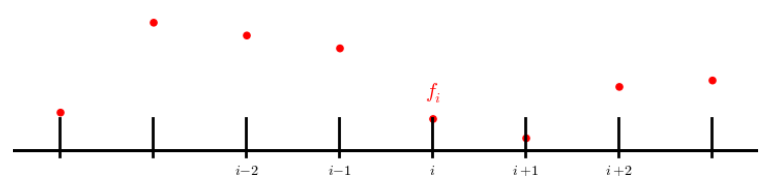
\includegraphics[width=30em]{13-22-29.png}

Sonlu hacim (FV) yönteminde durum biraz farklı; bir fonksiyonu belli
noktalarındaki noktasal değerlerle değil, belli aralıklar arasında kalan
değerlerinin averajı olarak temsil ediyoruz.

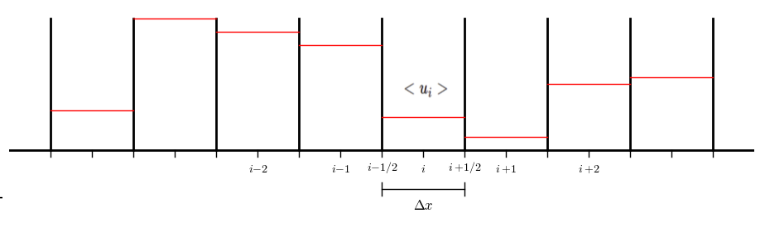
\includegraphics[width=30em]{13-22-34.png}

Üstteki görülen grafikte mesela $i$ ile $i+1$ noktası ortasındaki $i+1/2$
noktası ve $i$ ile $i-1$ noktası ortasındaki $i-1/2$ arasında kalan fonksiyonun
averajı alınacak, o zaman $<f_i>$ ya da $\bar{f}_i$

$$
\bar{f}_i = \frac{1}{\Delta x} \int _{x_{i-1/2}}^{x_{i+1/2}} f(x) \ud x
$$

Dikkat; $i-1,i-2$ değerleri $i$ referanslı olduğu için eksi içerikli, $i=4$
olsaydı onları 3,2 diye gidebilirdi. Ayrıca FD yönteminin aksine bu indis
değerlerine tekabül eden $x_i,x_{i+1}$ değerleri herhangi bir yerde olabilir,
böylece eşit aralıklı olmayan izgaralarla çalışmamız mümkün olur, bu FV
yönteminin kuvvetlerinden biridir.




[devam edecek]
  
Kaynaklar

[1] Zingale, {\em PHY 604: Computational Methods in Physics and Astrophysics II}


\end{document}
